\newpage
\section{Formal Defintion of PASS Process Models in OWL}
\label{OWL-DescriptionSID}



\begin{figure}[ht]
	\centering
	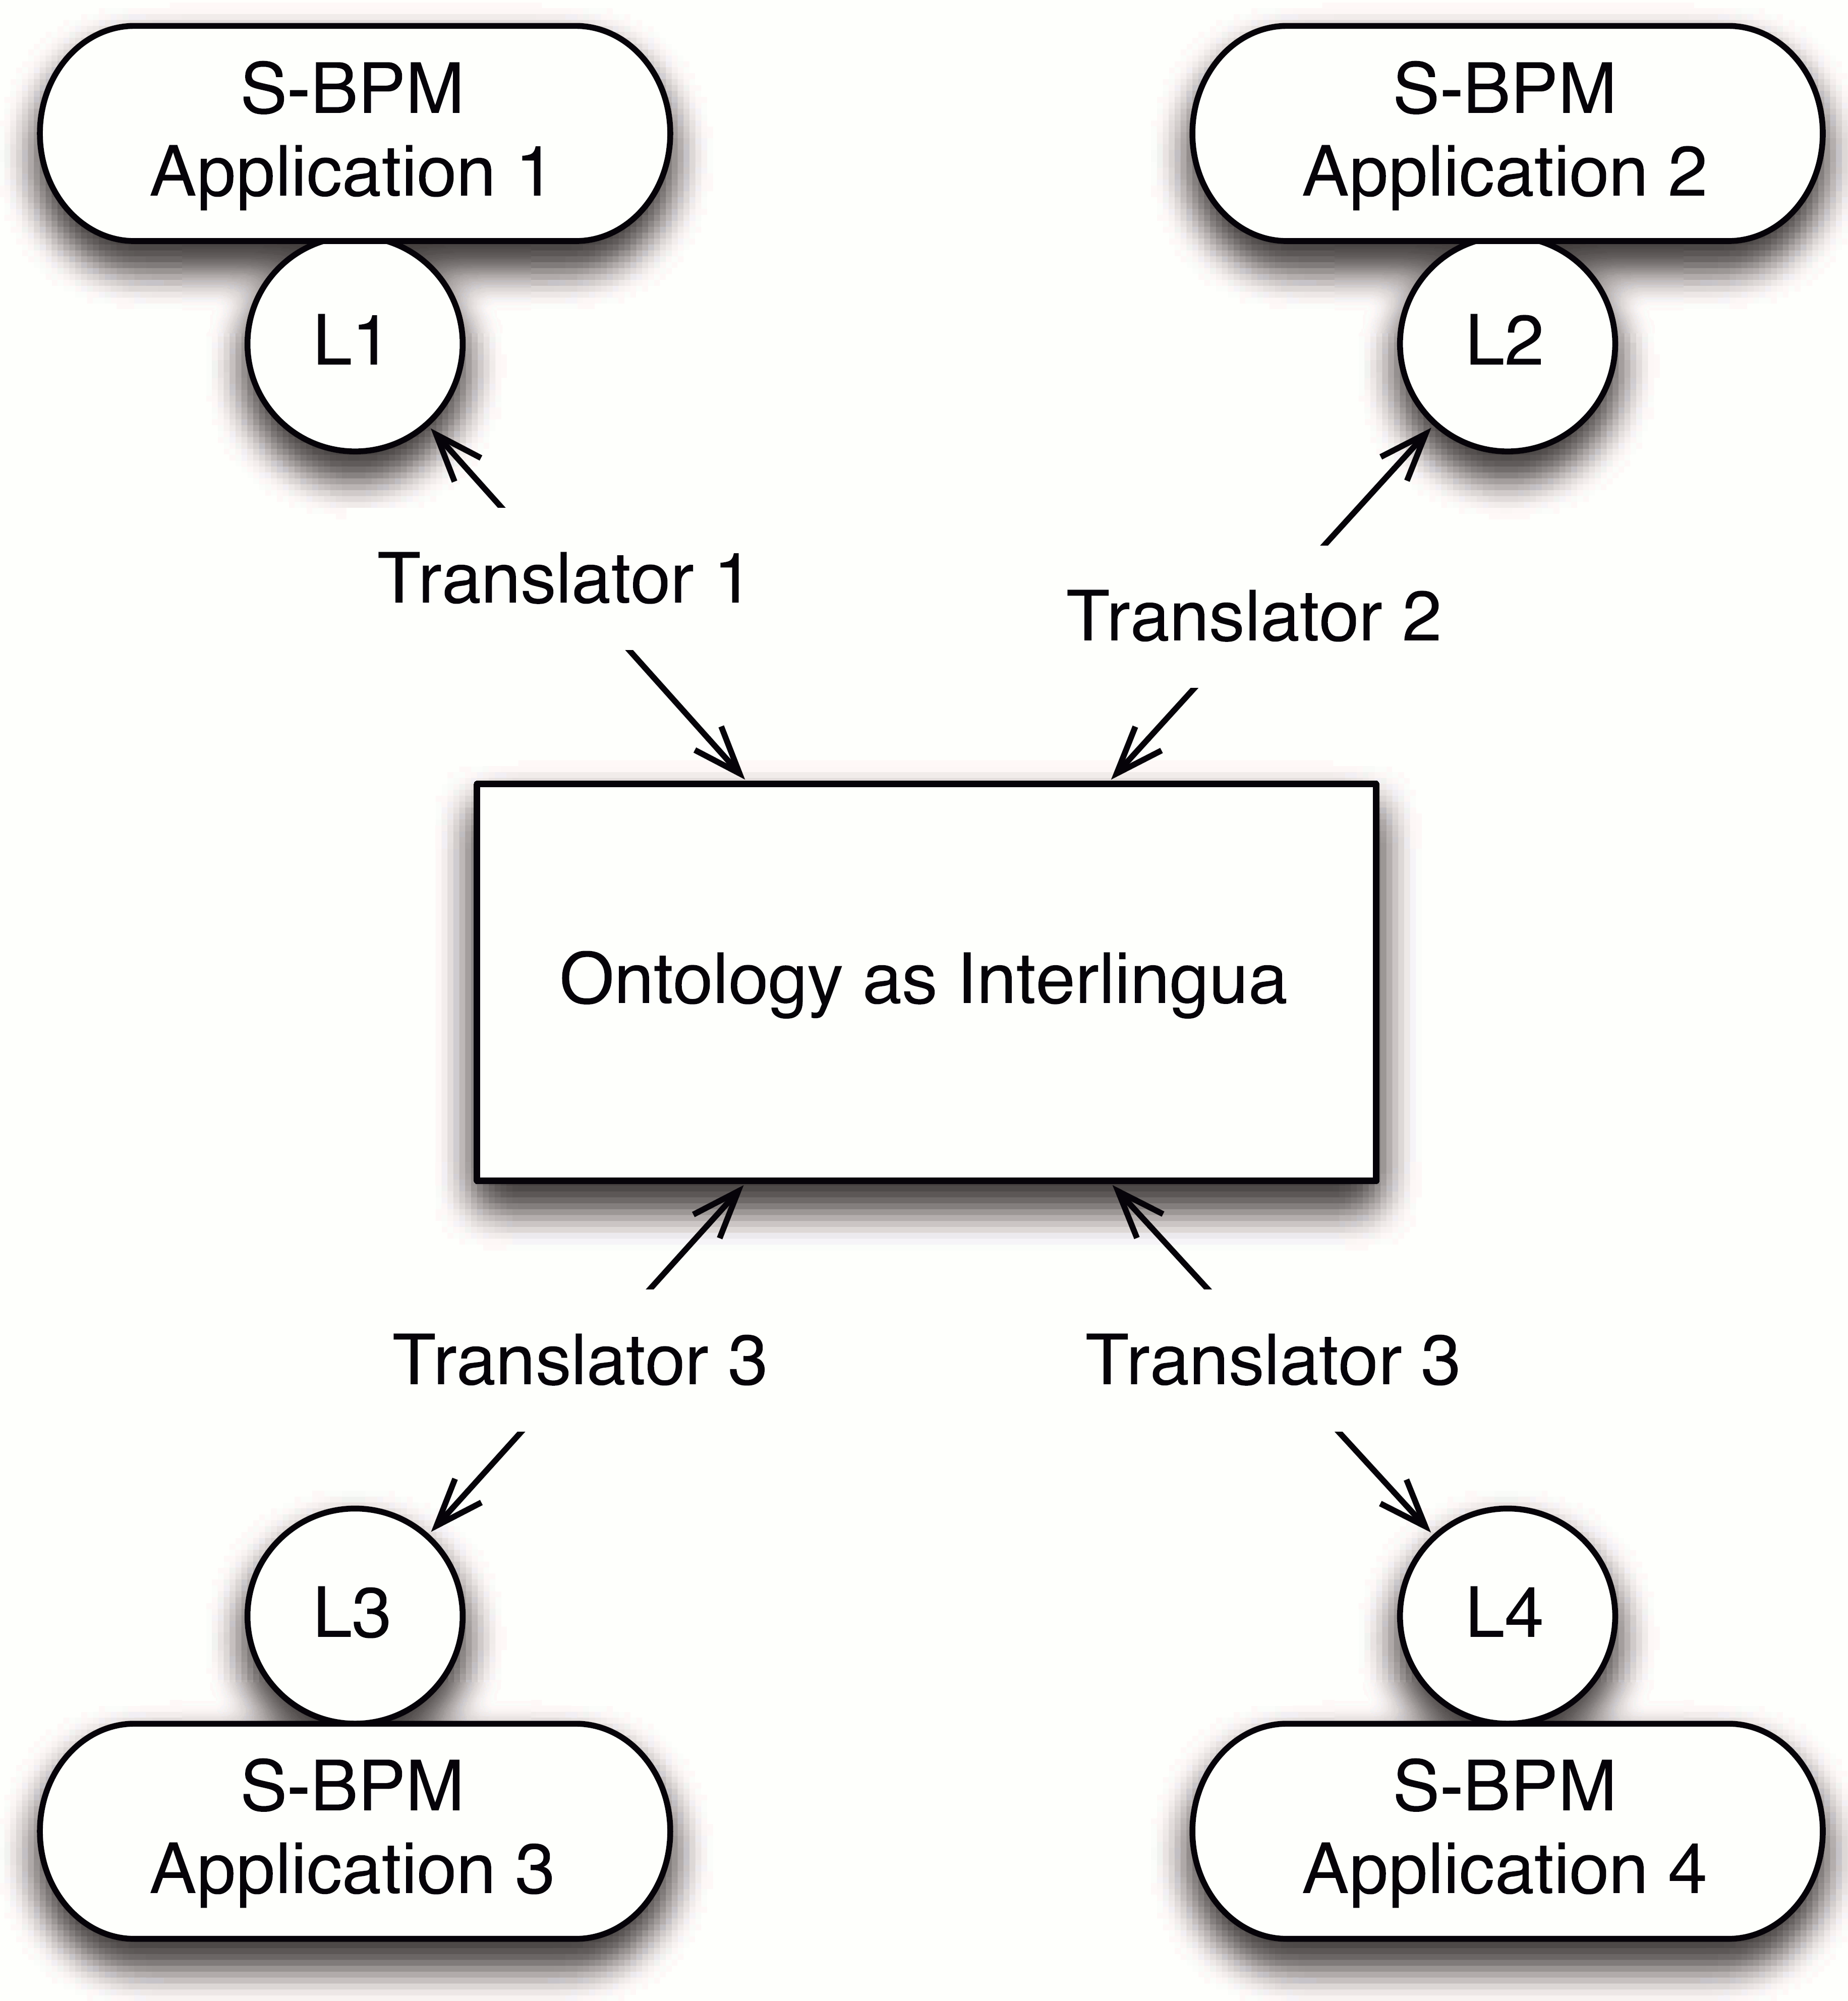
\includegraphics[width=0.50\textwidth]{Figures/Ontology/Introduction/hoeverproposal.png}
	\caption{Ontology as interchange format proposed by \cite{Hoever:ont}.}
\end{figure}


\subsection{Application Concept}

The Standard itself is formulated in OWL and will be available in an according \textit{standard-pass-ont.owl} file. The following Figure 2 taken from \cite{elster:ont} describes the application concept for how a process model should be saved in an individual model ontology file while referring to the standard definition ontology. At the same time an according model may refer to other ontological specifications that contain additional, but logically consistent and compatible, extensions to the standard.

\begin{figure}[ht]
	\centering
	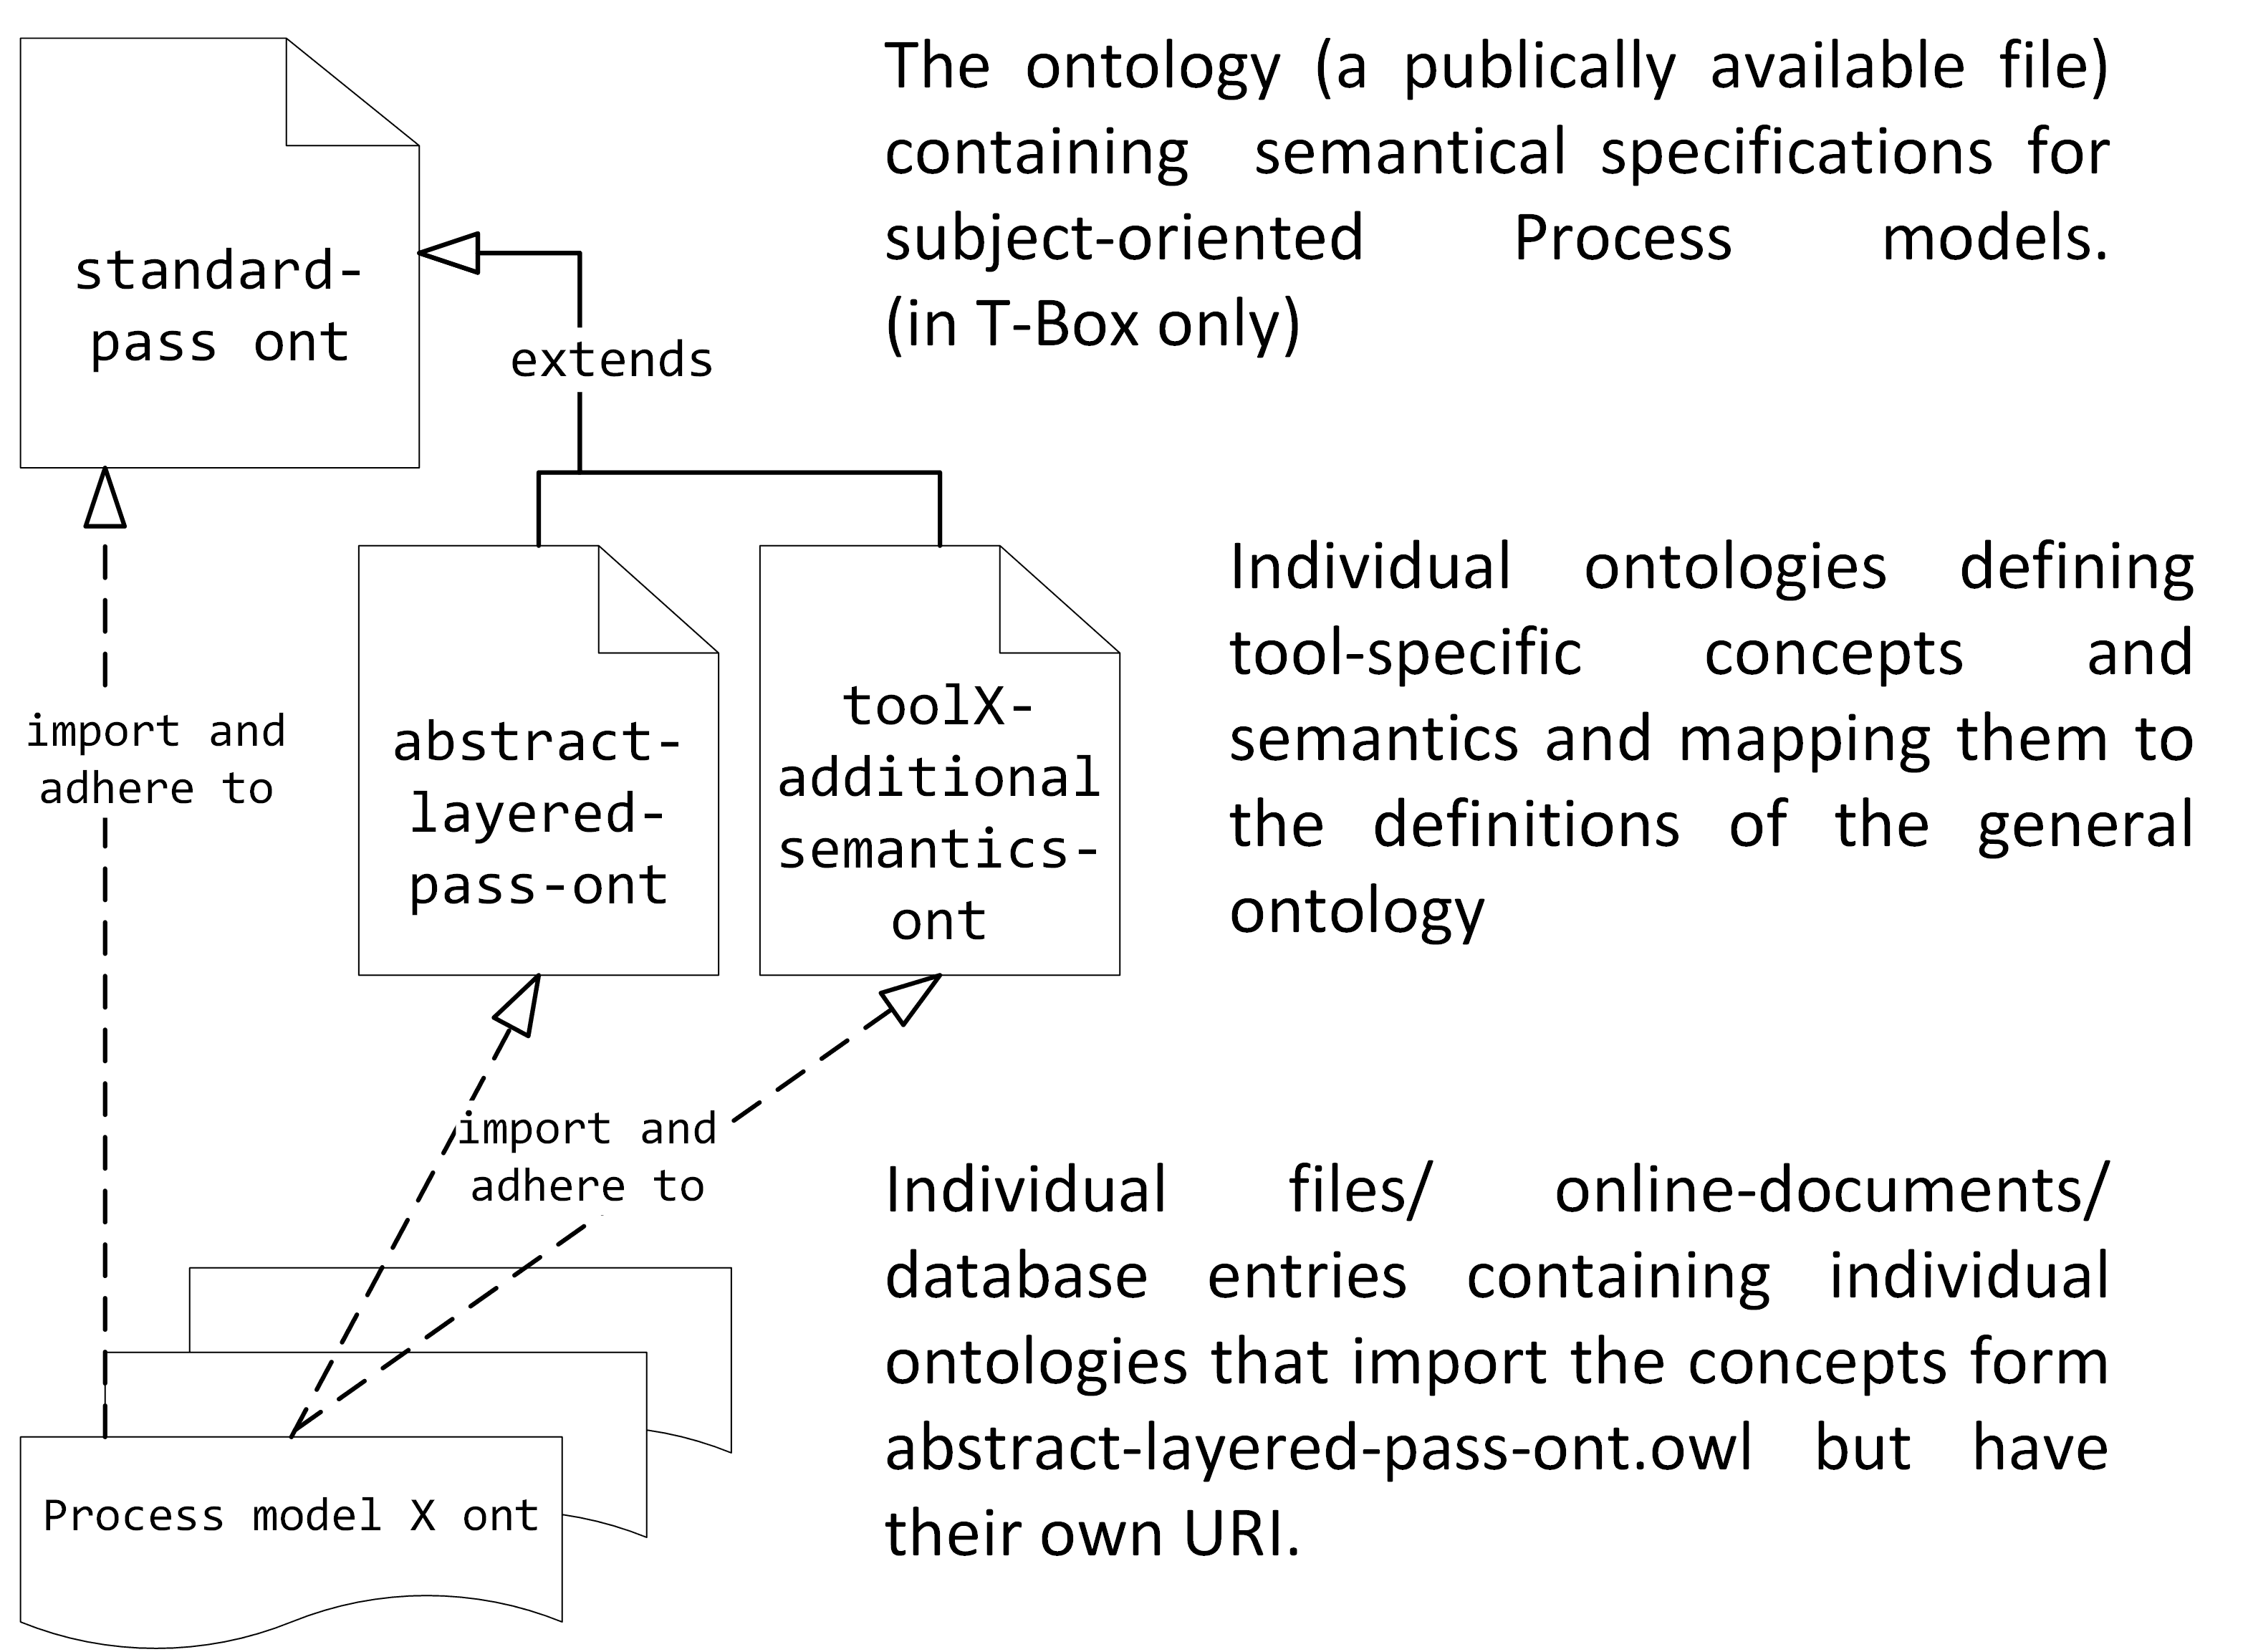
\includegraphics[width=0.50\textwidth]{Figures/Ontology/Introduction/ont-and-models.png}
	\caption{Proposed use and interaction of ontologies (from \cite{elster:ont} ).}
\end{figure}

\begin{figure}[ht]
	\centering
	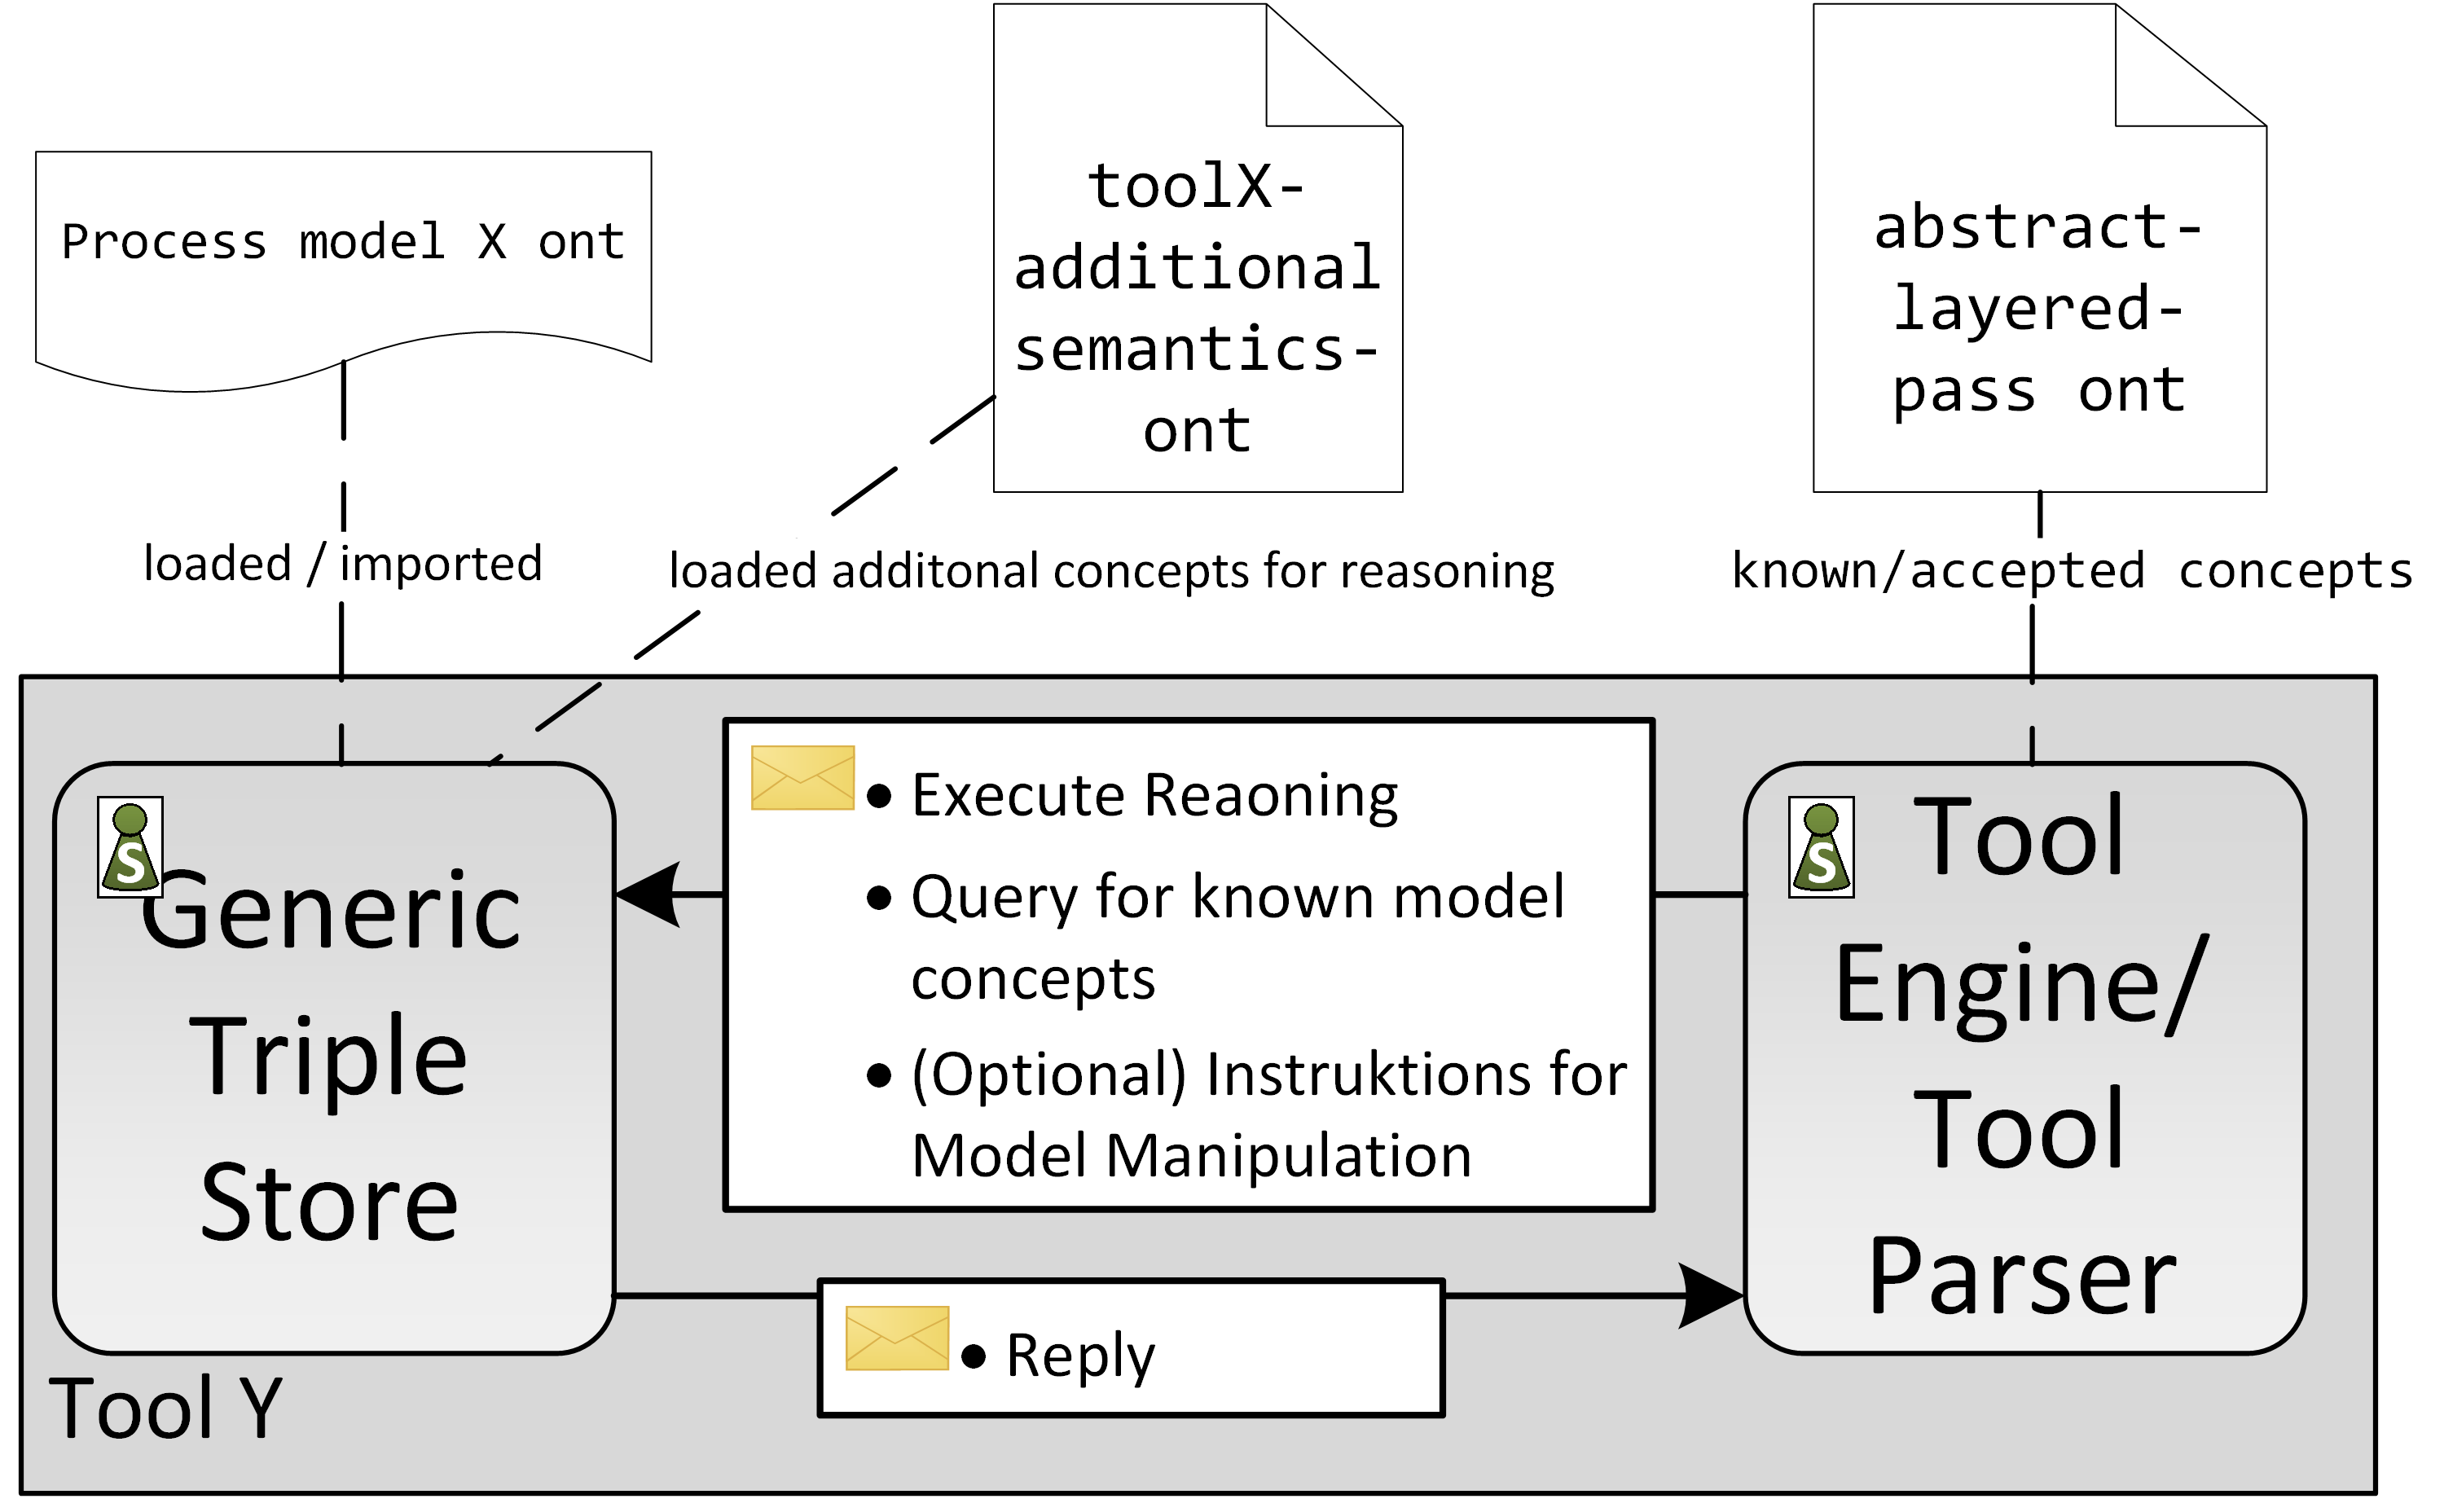
\includegraphics[width=0.50\textwidth]{Figures/Ontology/Introduction/importWorkflow.png}
	\caption{Conceptual Import Process (SID) (from \cite{elster:ont}). }
\end{figure}


\underline{\textit{\textbf{Übergang von informeller zur formalen Beschreibung sehr abrupt und unverstaändlich}}}


The various building blocks of a PASS description and their relations are defined in an ontology. The following figure \ref{fig:20171217-passprocessmodellelement} gives an overview of the structure of the PASS specifications.  

 
 \underline{\textit{\textbf{Nummerierung erklären, Wie kommen Nummern zustande}}}


\begin{figure*}[htbp]
	\centering
	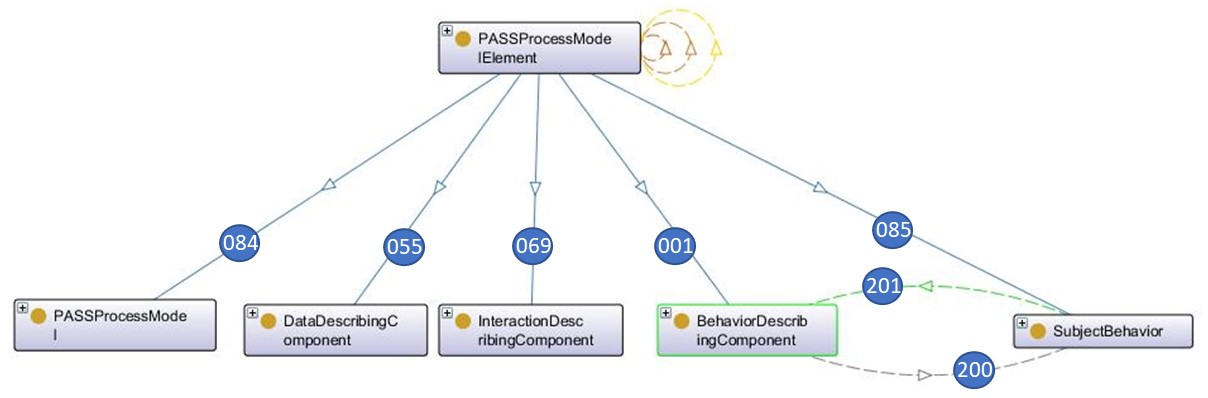
\includegraphics[width=0.9\linewidth]{Figures/Ontology/SubjectInteraction/20171217-PASSProcessModellElement}
	\caption[Elements of PASS Process Models]{Elements of PASS Process Models}
	\label{fig:20171217-passprocessmodellelement}
\end{figure*}

The class \texttt{PASSProcessModelElement} has five subclasses (subclass relations 084, 055, 069, 001 and 085 in figure \ref{fig:20171217-passprocessmodellelement}). Only the classes \texttt{PASSProcessModel}, \texttt{DataDescriptionCOmponent}, \texttt{InteractionDescribingComponent} are used for defining the structural aspects of a process specification in PASS. The classes \texttt{BehaviorDescribingComponent} and \texttt{SubjectBehavior} define the dynamic aspects, namely in which sequences messages are sent and received or internal actions are executed. These dynamic aspects are considered in detail in the next chapter. 

\subsection{PASS Process Model}

The central entities of a PASS process model are subjects which represent the active elements of a process and the messages they exchange. Messages transport data from one subject to others (payload). Figure \ref{fig:20181217-passprocessmodel} shows the corresponding ontology for the PASS process models.

\begin{figure*}[htbp]
	\centering
	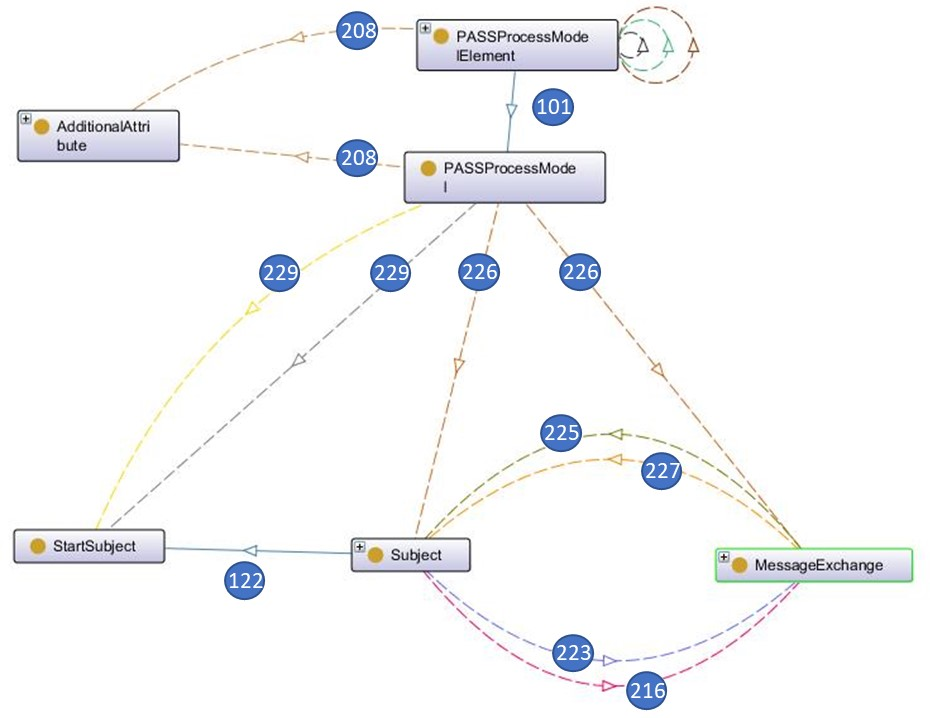
\includegraphics[width=1.0\linewidth]{Figures/Ontology/SubjectInteraction/20181217-PASSProcessModel}
	\caption[PASS Process Modell]{PASS Process Modell}
	\label{fig:20181217-passprocessmodel}
\end{figure*}

\texttt{PASSProcessModelElements} and \texttt{PASSProcessModells} have a name. This is described with the property \texttt{hasAdditionalAttribute} (property 208 in \ref{fig:20171217-passprocessmodellelement}). The class subject and the class \texttt{MessageExchange} have the relation \texttt{hasRelation} \texttt{toModelComponent} to the class \texttt{PASSProcessModel} (property 226 in \ref{fig:20171217-passprocessmodellelement}). The properties \texttt{hasReceiver} and \texttt{hasSender} express that a message has a sending and receiving subject (properties 225 and 227 in \ref{fig:20171217-passprocessmodellelement}) whereas the properties \texttt{hasOutgoingMessageExchange} and \texttt{hasIncomingMessageExchange} define which messages are sent or received by a subject. Property \texttt{hasStartSubject} (property 229 in \ref{fig:20171217-passprocessmodellelement}) defines a start subject for a \texttt{PASSProcessModell}. A start subject is a subclass of the class subject (subclass relation 122 in \ref{fig:20171217-passprocessmodellelement}).

\subsection{Data Describing Component}

Each subject encapsulates data (business objects). The values of these data elements can be transferred to other subjects. The following figure \ref{fig:20181218-data} shows the ontology of this part of the PASS-ontology.

\begin{figure}[htbp]
	\centering
	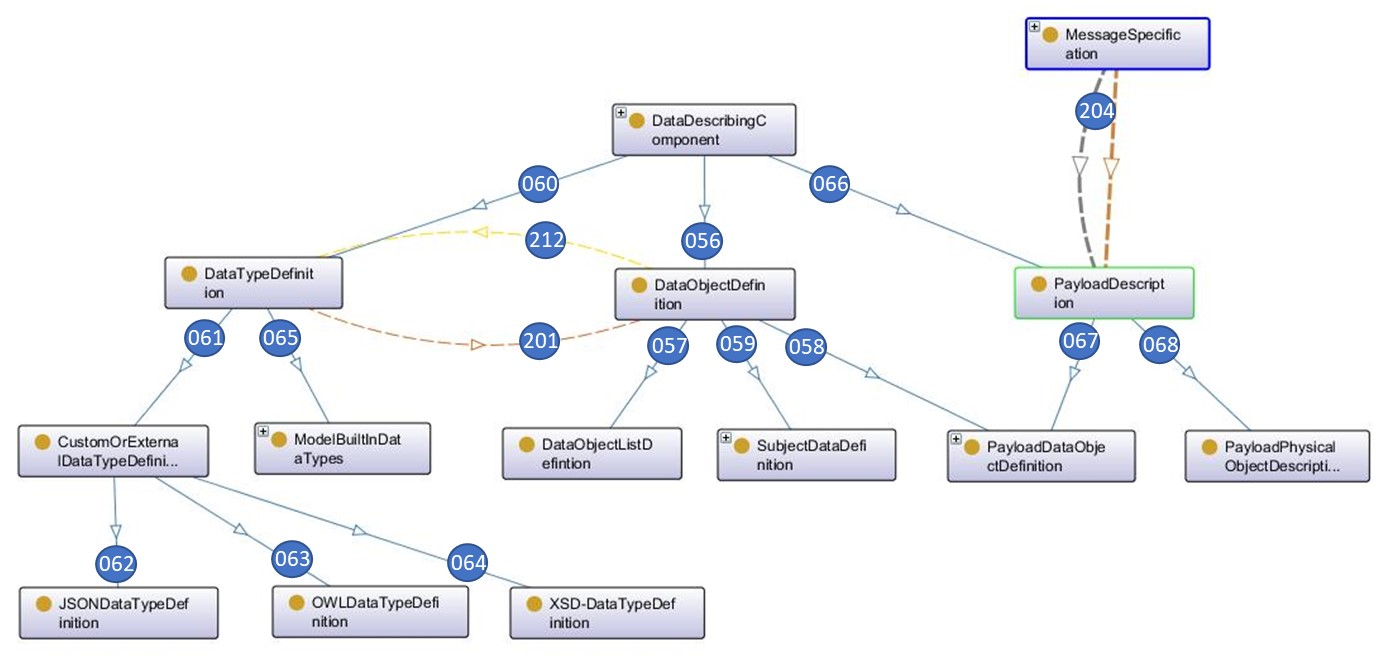
\includegraphics[width=0.9\linewidth]{Figures/Ontology/SubjectInteraction/20181218-Data}
	\caption[Data Description Component]{Data Description Component}
	\label{fig:20181218-data}
\end{figure}

Three subclasses are derived from the class \texttt{DtadescribingComponent} (in figure \ref{fig:20181218-data} are these the relations 060, 056 and 066). The subclass \texttt{PayLoadDescription} defines the data tranported by messages. The relation of \texttt{PayloadDescriptions} to messages is defined by the property \texttt{ContainsPayloadDescription} (in figure \ref{fig:20181218-data} number 204).

There are two types of payloads. The class \texttt{PayloadPhysicalObjectDescription} is used if a message will be later implemented by a physical transport like a parcel. The class \texttt{PayLoadDataObjectDefinition} is used to transport normal data (Subclass relations 068 and 67 in figure \ref{fig:20181218-data}). These payload objects are also a subclass of the class \texttt{DataObjectDefinition} (Subclass relation 058 in figure \ref{fig:20181218-data}).

Data objects have a certain type. Therefore class \texttt{DataObjectDefinition} has the relation \texttt{hasDatatype} to class \texttt{DataTypeDefinition} (property 212 in figure\ref{fig:20181218-data}). Class \texttt{DataTypeDefinition} has two subclasses (subclass relations 061 and 065 in figure \ref{fig:20181218-data}). The subclass \texttt{ModelBuiltInDataTypes} are user defined data types whereas the class \texttt{CustomOfExternalDataTypeDefinition} is the superclass of JSON, OWL or XML based data type definitions(subclass relations 062, 63 and 064 in figure \ref{fig:20181218-data}).

\subsection{Interaction Describing Component}

The following figure \ref{fig:ontogrsubjectinteraction} shows the subset of the classes and properties required for describing the interaction of subjects. 

\begin{figure*}[htbp]
	\centering
	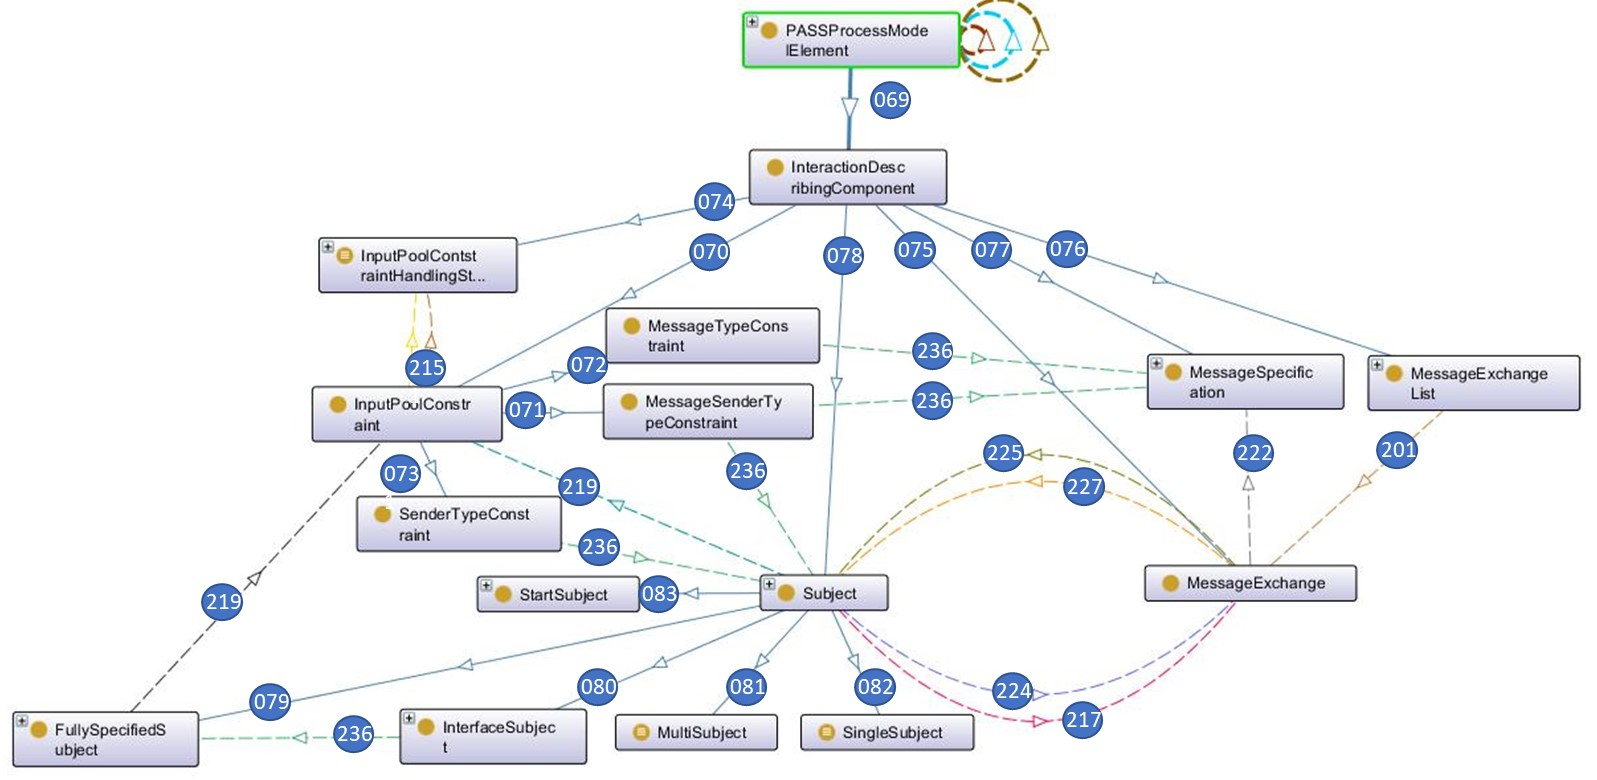
\includegraphics[width=1.0\linewidth]{Figures/Ontology/SubjectInteraction/OntoGrSubjectInteraction}
	\caption[Subject Interaction Diagram]{Subject Interaction Diagram}
	\label{fig:ontogrsubjectinteraction}
\end{figure*}

The central classes are \texttt{Subject} and \texttt{MessageExchange}. Between these classes are defined the properties \texttt{hasIncomingTransition} (in figure \ref{fig:ontogrsubjectinteraction} number 217) and \texttt{hasOutgoingTransition} (in figure \ref{fig:ontogrsubjectinteraction} number 224). These properties define that subjects have incoming and outgoing messages. Each message has a sender and a receiver (in figure \ref{fig:ontogrsubjectinteraction} number 227 and number 225). Messages have a type. This is expressed by the property \texttt{hasMessageType} (in figure \ref{fig:ontogrsubjectinteraction} number 222). Instead of the property 222 a message exchange may have the property 201 if a list of messages is used instead of a single message.

Each subject has an input pool. Input pools have three types of constraints (see section \ref{sec: inputpool}). This is expressed by the property references  (in figure \ref{fig:ontogrsubjectinteraction} number 236) and \texttt{InputPoolConstraints} (in figure \ref{fig:ontogrsubjectinteraction} number 219). Constraints which are related to certain messages have references to the class \texttt{MessageSpecification}.

There are four subclasses of the class \texttt{subject} (in figure \ref{fig:ontogrsubjectinteraction} number 079, 080, 081 and 082). The specialties of these subclasses are described in section \ref{sec: Subject}. A class \texttt{StartSubject} (in figure \ref{fig:ontogrsubjectinteraction} number 83) which is a subclass of class subject denotes the subject in which a process instance is started.

All other relations are subclass relations. The class \texttt{PASSProcessModelElement} is the central PASS class. From this class, all the other classes are derived (see next sections). From class \texttt{InteractionDescribingComponent} all the classes required for describing the structure of a process system are derived.

\section{ASM Description}

In this chapter, only the structure of a PASS model is considered. Execution has not been considered. Because ASM only considers execution aspects in this chapter an ASM specification of the structural aspects does not make sense. The execution semantics is part of chapter 4.


\section{Ontology of Subject Behavior Description}

Each subject has a base behavior (see property 202 in \ref{fig:20190104-simple-elements-and-modellelement}) and may have additional subject behaviors (see class \texttt{SubjectBehavior} in \ref{fig:20190104-simple-elements-and-modellelement}) for macros and guards. All these behaviors are subclasses of the class \texttt{SubjectBehavior}. The details of these behaviors are defined as state transition diagrams (PASS behavior diagrams). These behavior diagrams are represented in the ontology with the class \texttt{BehaviorDescribingComponent} (see figure \ref{fig:20190104-simple-elements-and-modellelement}). The behavior diagrams have the relation \texttt{belongsTo} to the class \texttt{SubjectBehavior}. The other classes are needed for \texttt{embeddingsubjects} into the subject interaction diagram (SID) of a PASS specification (see chapter \ref{OWL-DescriptionSID}).

\begin{figure}[htbp]
	\centering
	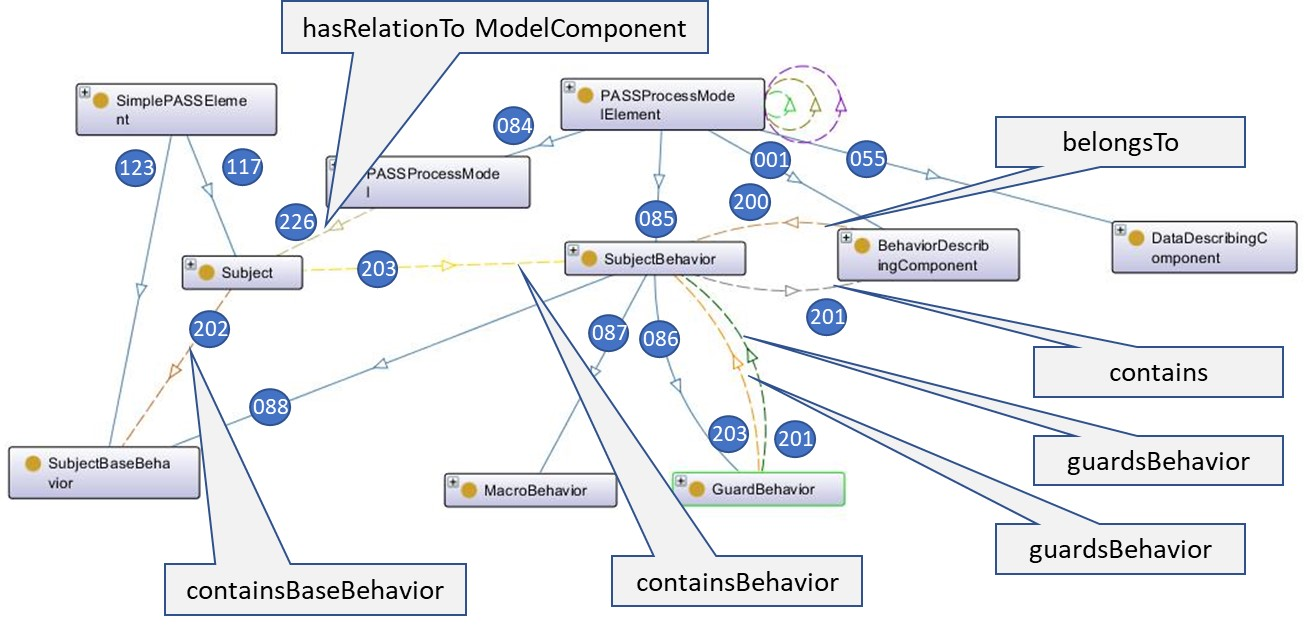
\includegraphics[width=0.9\linewidth]{Figures/Ontology/SubjectBehavior/20190104-SImple-Elements-and-Modellelement}
	\caption[Structure of Subject Behavior Specification]{Structure of Subject Behavior Specification}
	\label{fig:20190104-simple-elements-and-modellelement}
\end{figure}

\subsection{Behavior Describing Component}

The following figure shows the details of the class \texttt{BehaviorDescribingComponent}. This class has the subclasses State, Transition and \texttt{TranssitionCondition} (see figure \ref{fig:20190104-behavior-describing-component}). The subclasses of the state represent the various types of states (class relations 025, 014 and 024 in \ref{fig:20190104-behavior-describing-component}). The standard states \texttt{DoSTates}, \texttt{SendState} and \texttt{ReceiveState} are subclasses of the class \texttt{StandardPASSState} (class relations 114, 115 and 116 in \ref{fig:20190104-behavior-describing-component}). The subclass relations 104 and 020 allow that there exists a start state (class \texttt{InitialStatOfBehavior} in \ref{fig:20190104-behavior-describing-component}) and none or several end states (see subclass relation 020 in figure\ref{fig:20190104-behavior-describing-component}) The fact that there must be at least one start state and none or several end states is defined by so called axioms which are not shown in figure \ref{fig:20190104-behavior-describing-component}.

\begin{figure}[htbp]
	\centering
	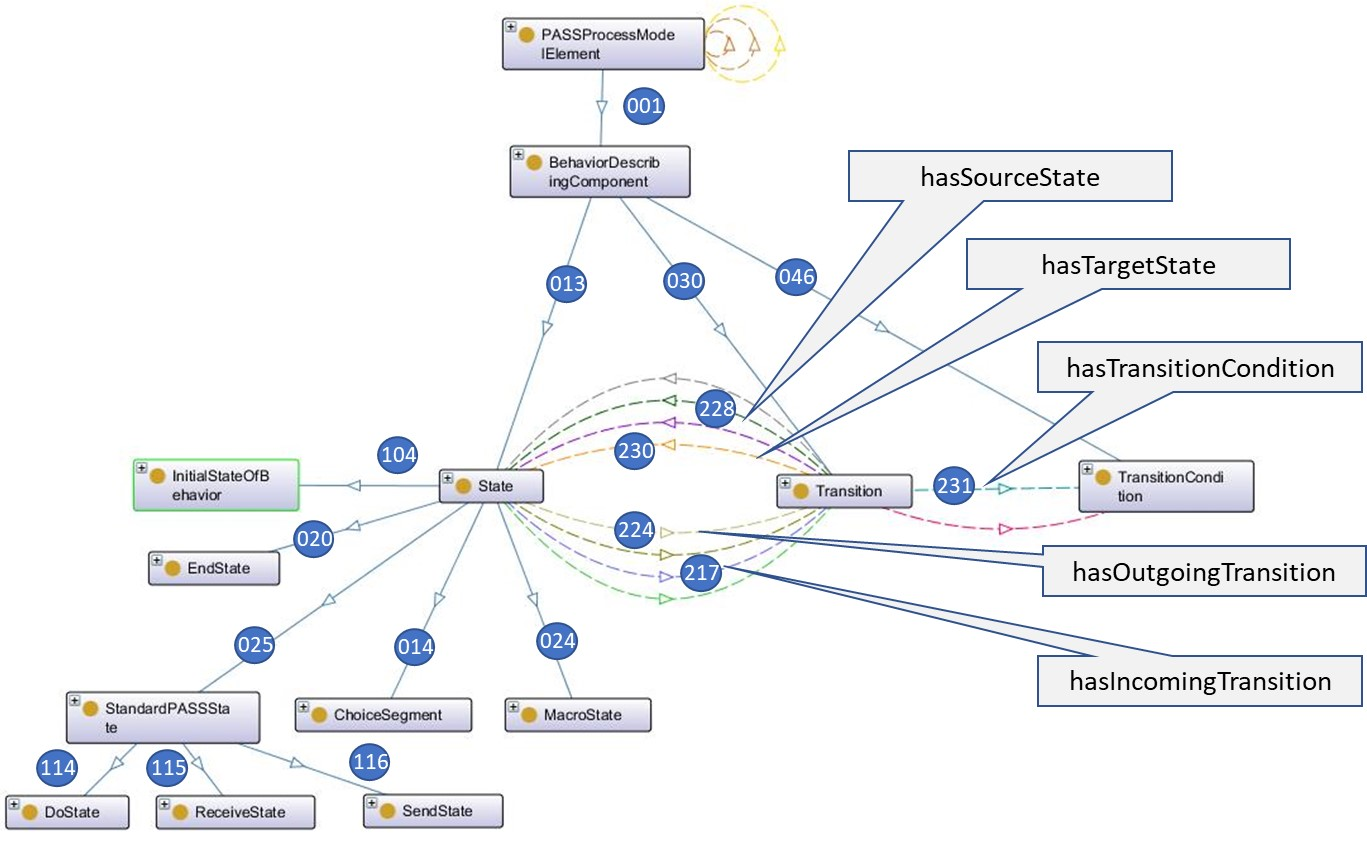
\includegraphics[width=1.0\linewidth]{Figures/Ontology/SubjectBehavior/20190104-Behavior-describing-component}
	\caption[Subject Behavior describingComponent]{Subject Behavior describingComponent}
	\label{fig:20190104-behavior-describing-component}
\end{figure}

States can be starting and/or endpoints of transitions (see properties 228 and 230 in figure \ref{fig:20190104-behavior-describing-component}). This means a state may have outgoing and/or incoming transitions (see properties 224 and 217 in figure \ref{fig:20190104-behavior-describing-component}). Each transition is controlled by a transition condition which must be true before a behavior follows a transition from the source state to the target state.

\subsubsection{States}

As shown in figure \ref{fig:20190109-states} the class state has a subclass \texttt{StandardPASSState} (subclass relation 025) which have the subclasses \texttt{ReceiveState}, \texttt{SendState} and \texttt{DoState}(subclass relations 027, 026, 025). A state can be a start state (subclass \texttt{InitialStateOfBehavior} subclass relation 022). Besides these standard states there are macro states (subclass 024). Macro states contain a reference (subclass 029) to the corresponding macro (Property 201).

\begin{figure}[htbp]
	\centering
	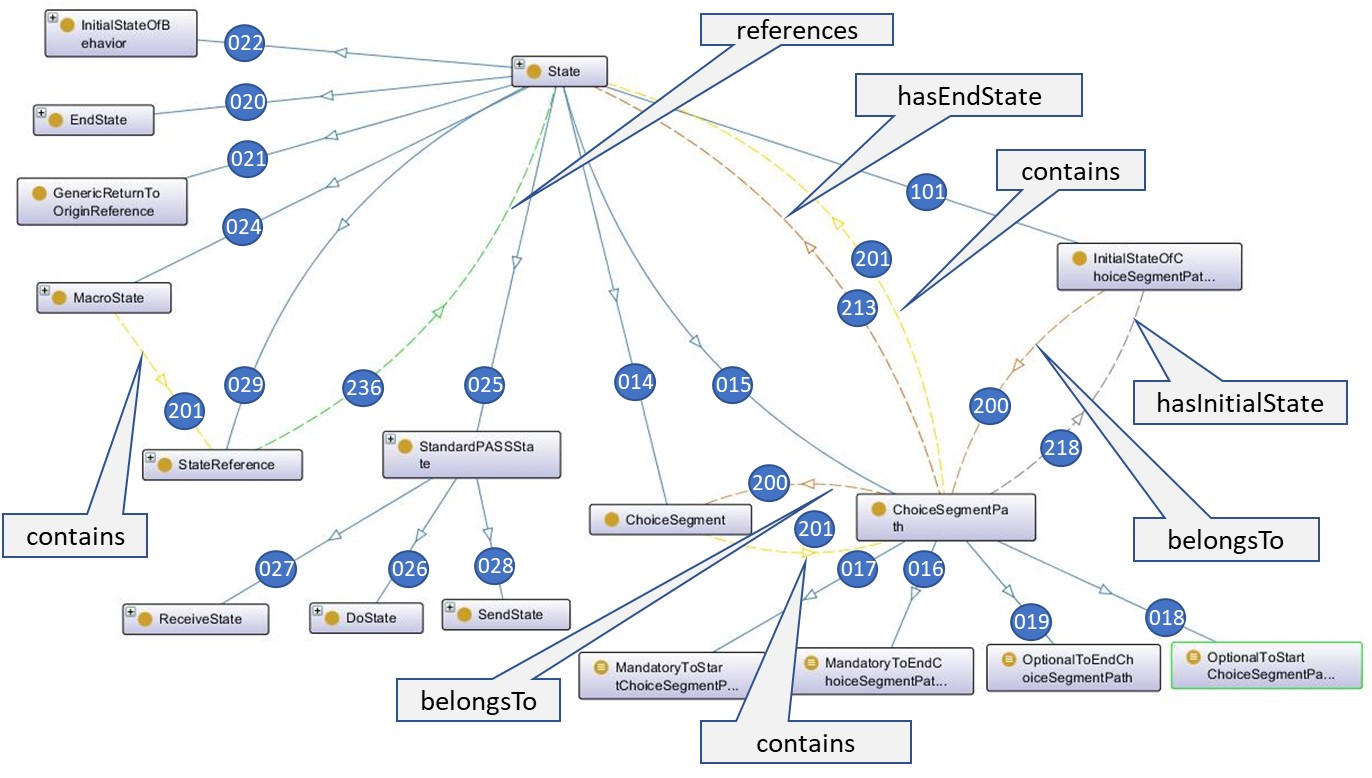
\includegraphics[width=1.0\linewidth]{Figures/Ontology/SubjectBehavior/20190109-States}
	\caption[Details of States]{Details of States}
	\label{fig:20190109-states}
\end{figure}

More complex states are choice segments (subclass relation 014). A choice segment contains choice segment paths (subclass 015 and property 200). Each choice segment path can be of one of four types. If a segment path is started then it must be finished or not, or a segment path must be started and must be finished or not (subclass relations 16, 17, 18 and 19).

\subsubsection{Transitions}

Transitions connect the source state with the target state (see figure \ref{fig:20190104-behavior-describing-component}). A transition can be executed if the transition condition is valid. This means the state of a behavior changes from the current state which is the source state to the target state. In PASS there are two basic types of transitions, \texttt{DoTransitions} and \texttt{CommunicationTranstions} (subclasses 34 and 31 in figure \ref{fig:20190105-transitions}). The class \texttt{CommunicationTransition} is divided into the subclasses \texttt{ReceiveTransition} and \texttt{SendTransition} (subclasses 32 and 33 in figure \ref{fig:20190105-transitions}). Each transition has depending from its type a corresponding transition condition (property 231 in figure  \ref{fig:20190105-transitions}) which defines a data condition which must be valid in order to execute a transition.

\begin{figure}[htbp]
	\centering
	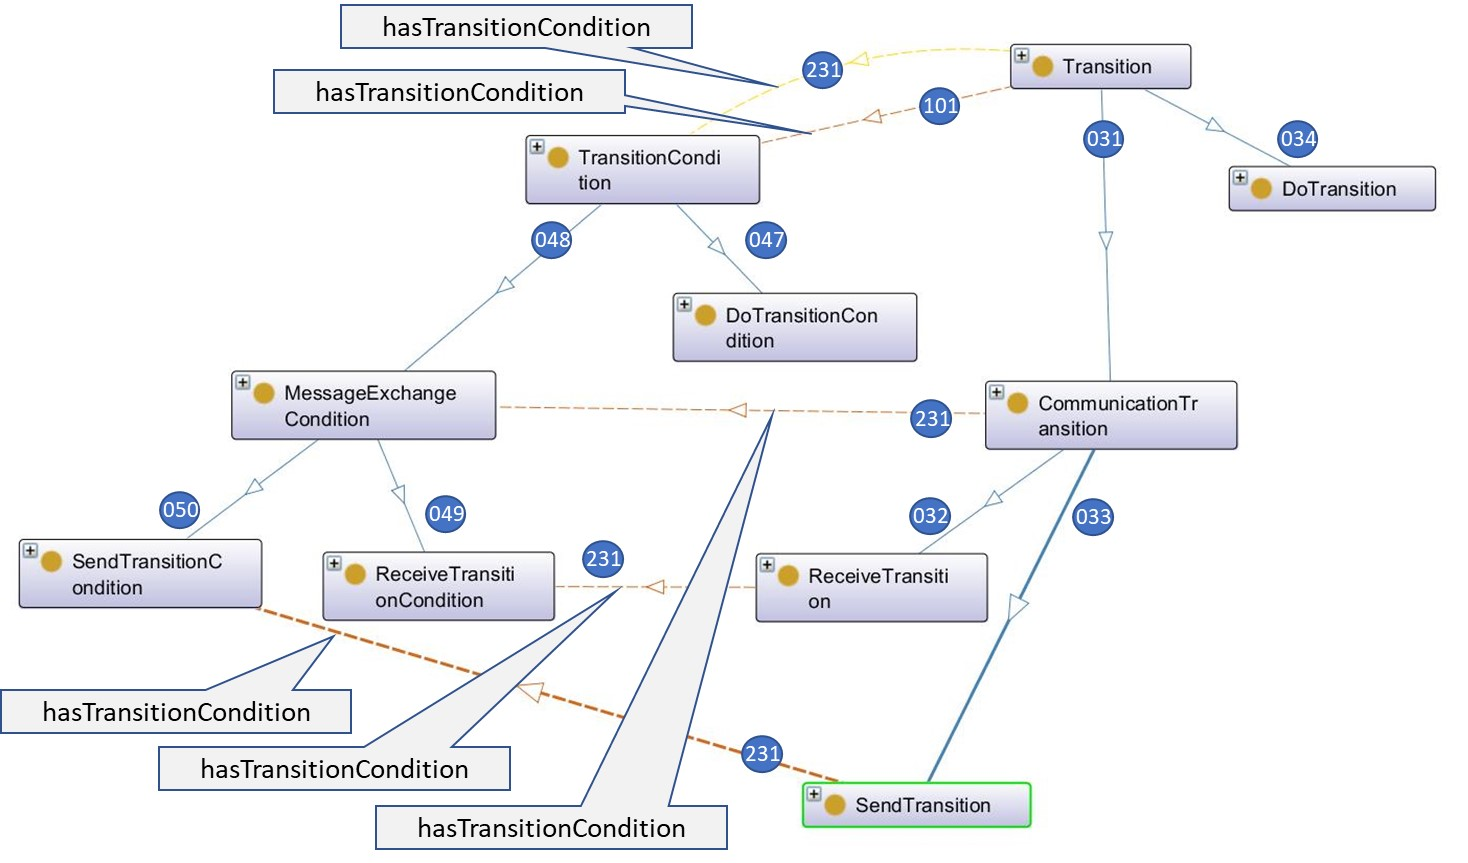
\includegraphics[width=1.0\linewidth]{Figures/Ontology/SubjectBehavior/20190105-Transitions}
	\caption[Details of transitions]{Details of transitions}
	\label{fig:20190105-transitions}
\end{figure}